The source and drain of an n-channel MOSFET are both formed by a metal-semiconductor junction with an n-type region in a p-type substrate. The gate is formed by placing an insulating oxide between a metal contact and the aforementioned p-type substrate. When a high voltage is applied at the gate, this attracts attracts excess electrons toward the gate. The electrons cannot leave the substrate due to the insulating oxide layer. So, they simply build up just below the oxide. The number of electrons in this region, known as the channel, increases considerably. However, by the principle of low-level injection ($\delta p \ll p$ under a perturbation, the applied voltage in this case), the number of holes in the p-type substrate does not change considerably. The conductivity of a semiconductor is given by equation (\ref{eq:cond_semi}):

\begin{equation}
	\label{eq:cond_semi}
	\sigma = q(\mu_n n + \mu_p p)
\end{equation}

Here, $\sigma$ is the conductivity, $q$ is the elementary charge, $\mu_n$ is the electron mobility, $\mu_p$ is the hole mobility, $n$ is the electron concentration, and $p$ is the hole concentration. Since $p$ does not change very much, but $n$ increases considerably, $\sigma$ increases. At a certain point, the channel essentially acts like a conductor. Electrons can now move freely between the source and drain terminals (1).

The situation is actually a bit more complicated. Depletion regions exist between the source and the gate and the gate and the drain. When $V_{GS}$ exceeds a threshold voltage, call it $V_{Th}$, the depletion region is overcome, much like in a pn-junction diode. Since the channel acts as a conductor, electrons, the majority carrier in the source, can now flow freely into the channel between the source and drain terminals. When $V_{GS} \leq V_{Th}$, the diode is "off" and is said to be in the cut-off region. The expected $I_D$ versus $V_{GS}$ plot is shown below. $I_D$ is essentially $0$ in the cut-off region and "turns on" after a certain threshold:

\FloatBarrier

\begin{figure}[h!]
	\centering
	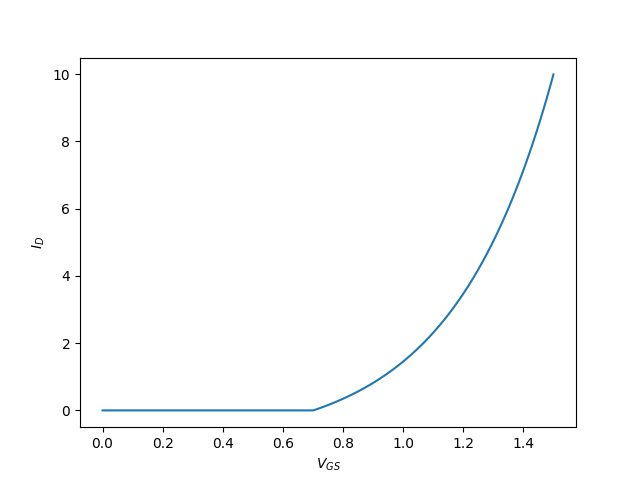
\includegraphics[scale=0.75]{./images/id_vs_vgs.PNG}
	\caption{Expected $I_D$ versus $V_{GS}$ Curve for an n-Channel MOSFET}
	\label{fig:id_vs_vgs}
\end{figure}

\FloatBarrier

Once the electrons have migrated from the source to the channel, the drain-source voltage, or $V_{DS}$ becomes important. Assume the MOSFET is in the "on" state in which $V_{GS} > V_{Th}$. The channel conductance is essentially constant and given by equation (\ref{eq:cond_semi}). Thus, the channel can be modeled as a simple resistor. By increasing $V_{D}$ and therefore $V_{DS}$, the drain can attract electrons more strongly, causing a greater electron current to flow from the drain. So, for small variations in $V_{DS}$, $I_{D}$ increases approximately linearly with $V_{DS}$. This is known as the triode region and occurs when $V_{DS} < V_{GS} - V_{Th}$.

However, this trend cannot continue indefinitely. At a certain point, electrons are so strongly attracted to the drain, that the channel loses many electrons, causing its conductivity to drop. This causes the drain current $I_{D}$ to taper off since the effect of attracting electrons to the drain by increasing $V_{DS}$ is counteracted by the drop in channel conductance. In integrated circuits, the channel width is small enough that the electrons are limited by velocity saturation, causing the same effect (2). This is known as the saturation region and occurs when $V_{GS} - V_{Th} < V_{DS}$ (3). However, with a sufficiently high $V_{DS}$, the voltage may be high enough to produce a strong enough electric field to force electrons from the source through the channel to the drain.

When $V_{GS}$ is increased, a greater electron current flows from the channel to the source. Therefore, the diode can operate in the triode region for longer because it can now draw a larger electron current from the drain to the channel. The saturation region still occurs, but at a higher drain current $I_D$. The expected plot is below with higher values of $V_{GS}$ reaching higher saturation drain currents $I_D$.

% Expected ID vs VDS

\FloatBarrier

\begin{figure}[h!]
	\centering
	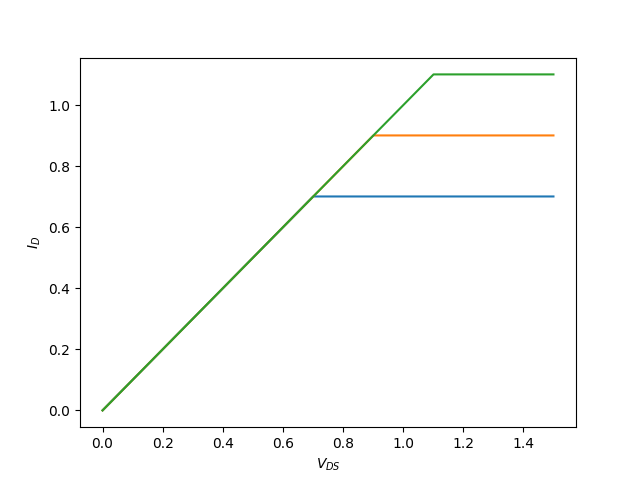
\includegraphics[scale=0.75]{./images/id_vs_vds.PNG}
	\caption{Expected $I_D$ versus $V_{DS}$ Curve for an n-Channel MOSFET}
	\label{fig:id_vs_vds}
\end{figure}

\FloatBarrier

If $V_{DS}$ is held constant and $V_{GS}$ is increased, eventually, $V_{DG}$ drops. If $V_{G}$ becomes sufficiently large relative to $V_{D}$, then the depletion region is not going to be strong enough to actually drive carrier electrons into the drain. So, a larger electron current flows from the channel, but the gate-drain depletion region resists the flow of electrons into the drain. These two effects balance one another out and cause the drain current to level off.

The circuit in figure (\ref{fig:mosfet_circ}) is used to plot the MOSFET curves.

\begin{figure}[h!]
\centering
\caption{MOSFET Measurement Circuit}
\label{fig:mosfet_circ}
\begin{circuitikz}
	\draw
	( 0 , 0 ) node[ nmos ] (my_nmos) {}
	(my_nmos.G) to [ R ] ++( -2 , 0 ) coordinate(r_in)
	(my_nmos.G) node[label={ [font=\normalsize] above : $V_{GS}$ } ] { }
	(r_in) to [ battery , v<=$V_1$ ] ++( 0 , -2 ) coordinate(gnd_1)
	(gnd_1) node[ ground ] (my_gnd_1) {}
	(my_nmos.S) node[ ground ] (my_gnd_2) {}
	(my_nmos.D) to [ R , i<_=$I_D$] ++( 0 , 2 ) coordinate(r_c)
	(my_nmos.D) node[label={ [font=\normalsize] below : $V_{DS}$ } ] { }
	(r_c) to [ battery , v<=$V_2$ ] ++( 2 , 0 ) coordinate(gnd_3)
	(gnd_3) node[ ground ] (my_gnd_3) {}
	;
\end{circuitikz}
\end{figure}

To acquire the $I_D$ versus $V_{GS}$ plot, $V_2$ is fixed at $10$\si{\volt}. $V_1$ is varied to observe different measurement points. It should be noted that because the oxide layer prevents current from flowing from the gate's metal contact to the substrate, no current flows through the gate. Thus, the gate voltage $V_G$ is simply $V_1$. Since the source is grounded, $V_S = 0$, which implies that $V_{GS} = V_G - V_S = V_G = V_1$. Thus, $V_1$ and therefore $V_{GS}$ is varied. As different $I_{D}$ values are observed, the measurements are noted until an $I_{D}$ versus $V_{GS}$ curve is obtained.
Note that gate voltages can be obtained by probing the pins in the MOSFET package. The current $I_D$ can be measured by taking the voltage drop over the resistor connected to the drain and applying Ohm's Law.

\FloatBarrier

\begin{table}[h!]
	\centering
	\caption{MOSFET $I_D$ versus $V_{GS}$ Data}
	\label{tab:mosfet_id_vgs}
	\csvautotabular{./tables/mosfet_id_vgs.csv}
\end{table}

\FloatBarrier

{\footnotesize $I_D$ is acquired by using Ohm's Law with the measured and not the reported resistance values. The resistor connected to the drain is measured to be 0.998\si{\kilo\ohm} and the resistor connected to the gate is 9.902\si{\kilo\ohm}. $V_2$ is fixed to $10$\si{\volt}.}

\FloatBarrier

\FloatBarrier

\begin{figure}[h!]
	\centering
	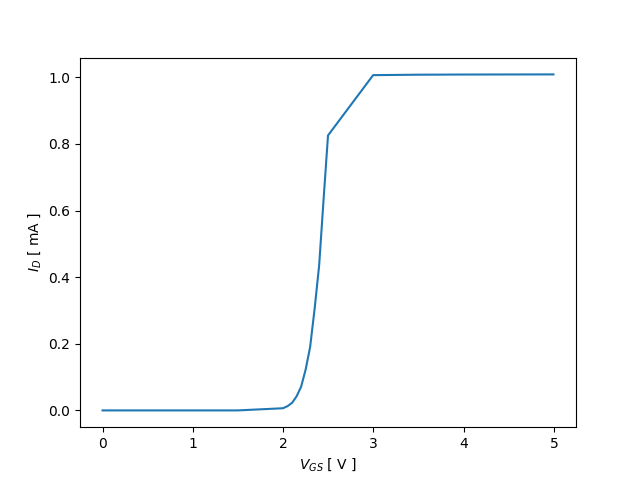
\includegraphics[scale=0.75]{./images/mosfet_id_vgs.PNG}
	\caption{MOSFET $I_D$ versus $V_{GS}$ Plot}
	\label{fig:mosfet_id_vgs}
\end{figure}

\FloatBarrier

The plot in figure (\ref{fig:mosfet_id_vgs}) is precisely as predicted. The MOSFET turns on when $V_{GS}$ exceeds the threshold voltage $V_{Th}$, which is slightly above $2$\si{\volt}. The drain current $I_{D}$ rises exponentially as $V_{GS}$ increases since a larger electron current can now be driven from the channel. Eventually, the curve levels off because the gate voltage $V_{G}$ becomes sufficiently large relative to the drain voltage $V_{D}$, which begins to counteract the flow of electrons into the drain.

To acquire the $I_D$ versus $V_{DS}$ plot, $V_1$ is fixed at about $2.3$\si{\volt}, which is around $V_{Th}$ for the MOSFET as predicted by the previous results. Thus, $V_{GS}$ is fixed. Increasing $V_2$ also increases the drain voltage $V_{D}$ and thus $V_{DS}$ since $V_{DS} = V_D - V_S = V_D$. Again, the drain current $I_D$ can be measured from the voltage over the drain's resistor and Ohm's Law.

\FloatBarrier

\begin{table}[h!]
	\centering
	\caption{MOSFET $I_D$ versus $V_{DS}$ Data}
	\label{tab:mosfet_id_vds}
	\csvautotabular{./tables/mosfet_id_vds.csv}
\end{table}

\FloatBarrier

{\footnotesize $V_1$ is fixed at $2.3$\si{\volt}.}

\FloatBarrier

\FloatBarrier

\begin{figure}[h!]
	\centering
	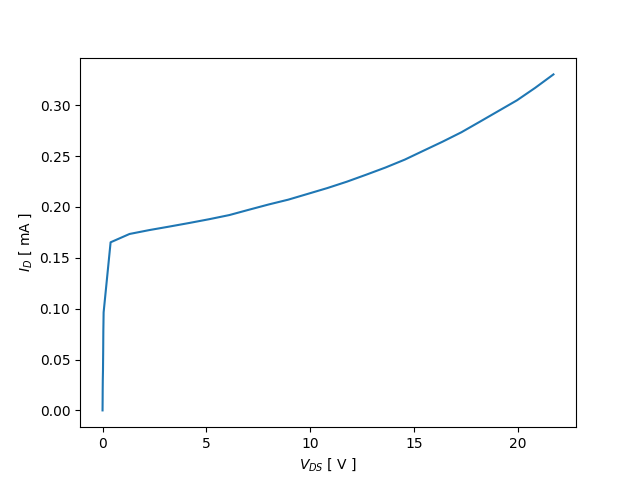
\includegraphics[scale=0.75]{./images/mosfet_id_vds.PNG}
	\caption{MOSFET $I_D$ versus $V_{DS}$ Plot}
	\label{fig:mosfet_id_vds}
\end{figure}

\FloatBarrier

The $I_D$ versus $V_{DS}$ curve is quite close to what is expected. The curve starts off linear when it is in the saturation region. The increased drain voltage relative to the source voltage is similar to increasing the voltage drop over an Ohmic resistor with the channel acting as the resistor. The voltage and current follow a linear relationship. The steepness of the curve reflects the low channel resistance. However, at a certain point, the drain voltage $V_{D}$ becomes very large relative to the gate voltage $V_{G}$. As a result, too many electrons flow to the drain, decreasing the channel's conductance and causing the curve to level off. The growth of the curve at the end is likely due to the very high voltage driving electrons to the drain as described above.

Because $V_1$ is fixed at $2.3$\si{\volt}, $V_{GS} = 2.3$\si{\volt}. The MOSFET operates in the triode region for $V_{DS} < V_{GS} - V_{Th} \approx 2.3$ \si{\volt} $ - 2$ \si{\volt} $ = 0.3$ \si{\volt} assuming $V_{Th} \approx 2$ \si{\volt}. The triode region, though visible, is quite short lived due to the fact that $V_{GS} - V_{Th}$ is only greater than $V_{DS}$ at the very beginning of the curve. As a result, it quickly enters the saturation region. Increasing $V_{GS}$ would prolong the triode region and possibly flatten out the curve afterward.
